\documentclass[11pt]{article}
\usepackage{amsmath,textcomp,amssymb,geometry,graphicx,float,mathrsfs,tabularx}

\def\Login{ee121-af} % Your login
\def\HW{3} % Homework number

\title{EE 121 -- Fall 2013\\Homework 2}

\markboth{EE 121 -- Fall 2013 Homework \HW}{EE 121 -- Fall 2013 Homework \HW}
\pagestyle{myheadings}

\begin{document}
\maketitle
\noindent\textbf{Team Bitdiddlers} \\
\text{Jeff Lievense, Rishi Sharma, Nader Behdin, Tim Brown}

\begin{enumerate}
  % Have a new \item for each problem
  % Make sure you have a \newpage after each item


  % PROBLEM 1
  \item
    \begin{enumerate}


        %part a)
        \item We generate a generator matrix row by row by creating a random bit string (length $k$) of Bernoulli Random Variables ($\mathcal{B}(\frac{1}{2})$) and appending them to our matrix $G$. The dot product of each row with the message (mod 2) is the parity bit for each row. We can decode when our generator matrix is full rank (i.e. we can solve a system of k equations), and the following plot shows an estimate of the PMF (generated by a normalized histogram) of $N$, number of rows necessary to decode a message of length $k=10$ and $k=100$ in 100 trials. See Figures 1 through 4.


        % part b)
        \item Now we generate rows of a generator matrix $G$ in the same fashion as before, but they are drawn from the ideal and robust soliton distribution. The encoding process is exactly the same as discussed in class. We choose a number $D$ from the Soliton distribution of choice. Then we randomly choose $D$ elements in a row of length $k$ and choose them to be 1's. Thus those $D$ elements will have their parity checked by the current row of the matrix being generated. We use the function sampleFromDist to sample from the Soliton distribution and then generateRow to create rows of the Matrix. In rateless.m we continuously generate rows of the matrix until we can successfully decode. The following are plots of the PMF's of $N$ for both the ideal and robust Soliton distribution, where $N$ is the number of rows of $G$ that must be generated before we can successfully decode using a linear equation solver (i.e. the matrix $G$ is full rank). See Figures 5 through 12.



        % part c)
        \item The function to solve a sparse system of equations by substitution only (found in substitutionSolver.m) implements an algorithm similar to that described in Luby's seminal paper on LT Codes. The substitution based solver has more strict conditions for solvability than simple linear equation solving, so it will require more rows from the parity check matrix to decode. We are willing to pay this price price for the linear time decoding granted by substitution decoding. Below are plots of the PMF's of $N$ for both the ideal and robust Soliton distribution, where $N$ is the number of rows of $G$ that must be generated before we can successfully decode using our substitution decoding algorithm. See Figures 13 through 20. \\
            \\
            Compared to parts (a) and (b), it takes noticeably more equations to be able to solve for the message bits, and as a result, the median and 90-percent quantile are greater. But, the decoding program runs \emph{much} faster.




        % part d)
        \item Although substitution based decoding requires more overall equations, linear time decoding allows us to decode for much larger values of $k$, whereas the linear equation solver simply takes too long to decode. Specifically, we were not able to generate plots for $k = 1000$ in parts (a) and (b), but after implemented the substitution-only-based solver, we were able to generate plots for $k = 1000$ in under a minute.

            \newpage




    \end{enumerate}


    \begin{figure}[H]
        \begin{center}
            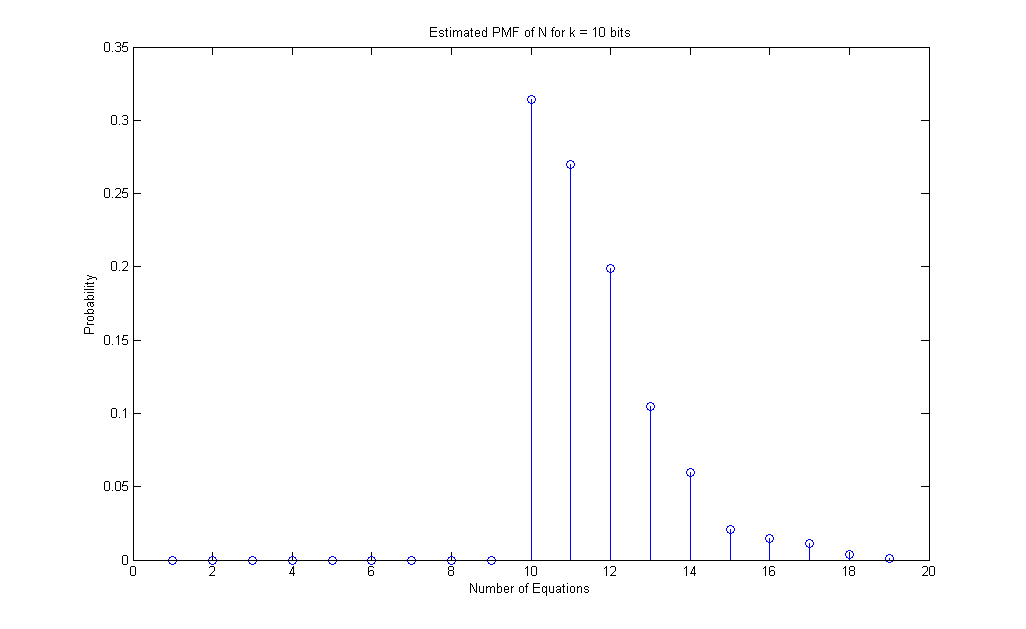
\includegraphics[width = 0.8\textwidth]{figure_1a_k10.png}
            \caption{Generic equation-solving with a uniform degree distribution.}
        \end{center}
    \end{figure}

    \begin{figure}[H]
        \begin{center}
            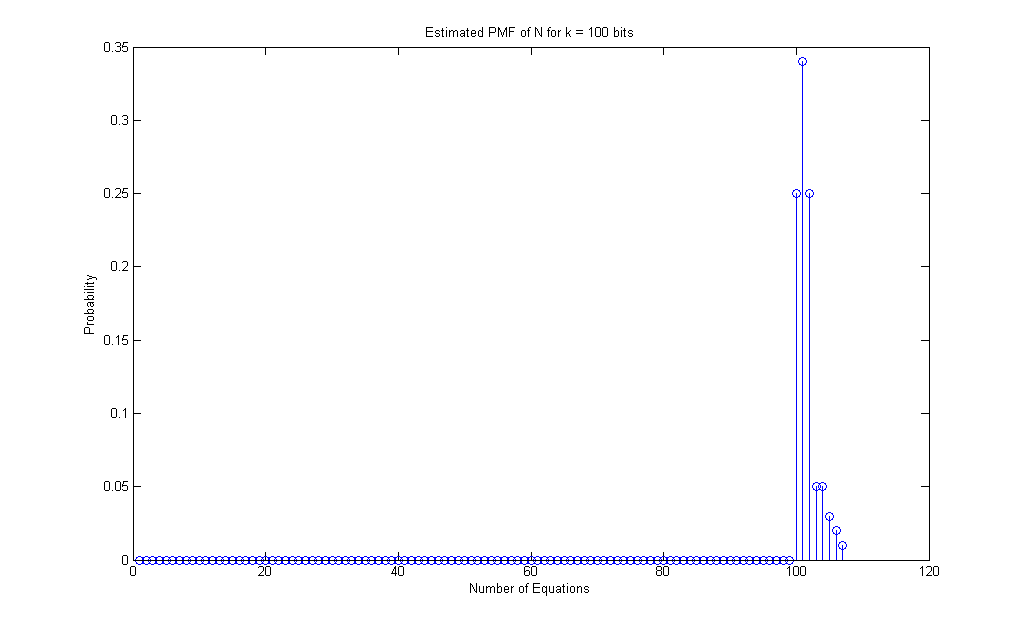
\includegraphics[width = 0.8\textwidth]{figure_1a_k100.png}
            \caption{Generic equation-solving with a uniform degree distribution.}
        \end{center}
    \end{figure}

    \begin{figure}[H]
        \begin{center}
            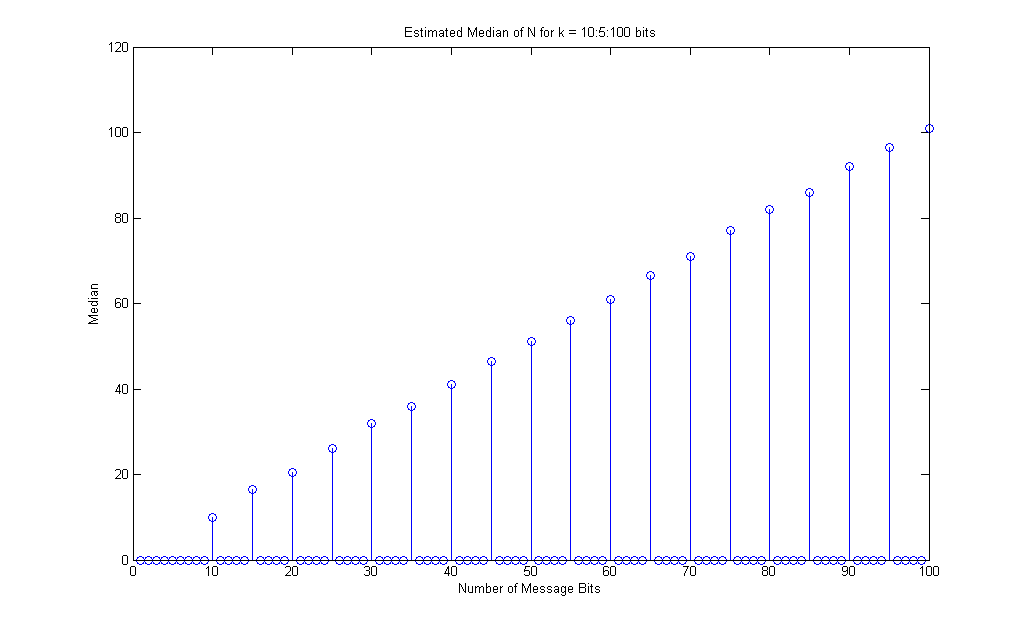
\includegraphics[width = 0.8\textwidth]{figure_1a_median.png}
            \caption{Generic equation-solving with a uniform degree distribution.}
        \end{center}
    \end{figure}

    \begin{figure}[H]
        \begin{center}
            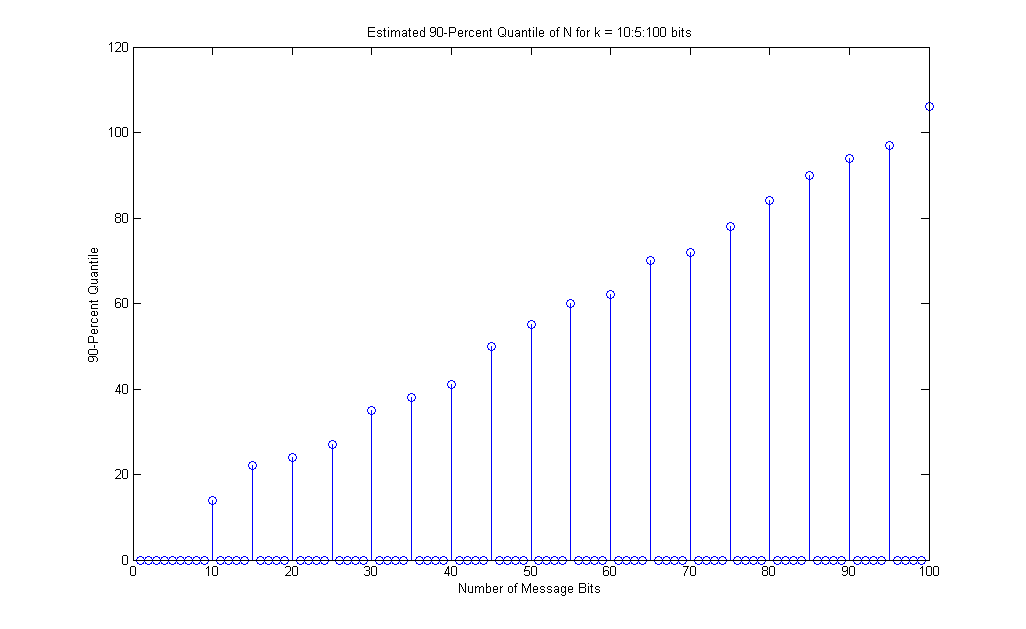
\includegraphics[width = 0.8\textwidth]{figure_1a_90_percent_quantile.png}
            \caption{Generic equation-solving with a uniform degree distribution.}
        \end{center}
    \end{figure}

    \begin{figure}[H]
        \begin{center}
            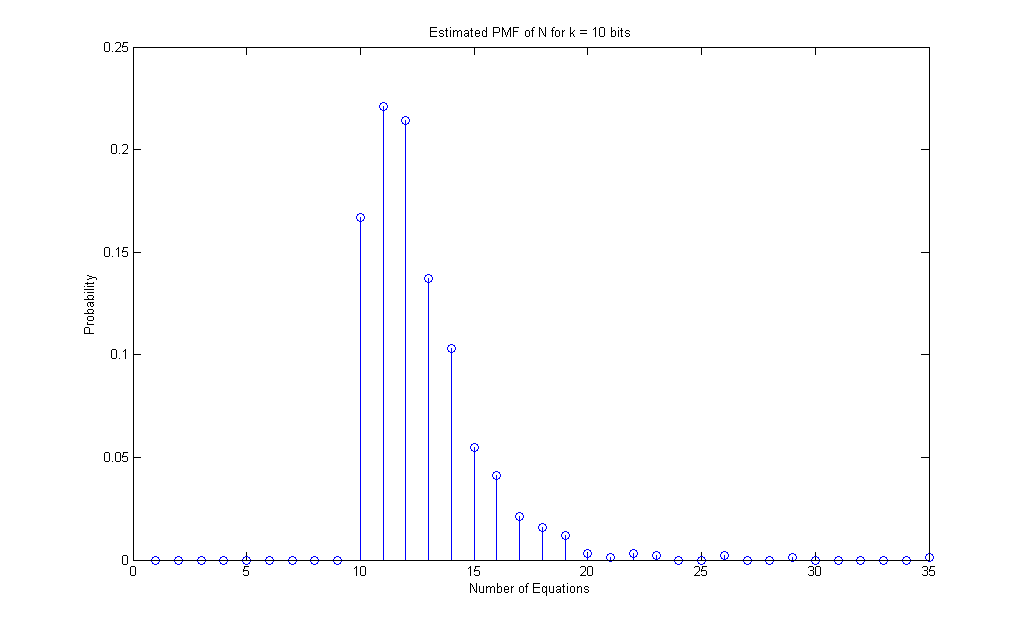
\includegraphics[width = 0.8\textwidth]{figure_1b_k10_ideal.png}
            \caption{Generic equation-solving with the Ideal Soliton degree distribution.}
        \end{center}
    \end{figure}

    \begin{figure}[H]
        \begin{center}
            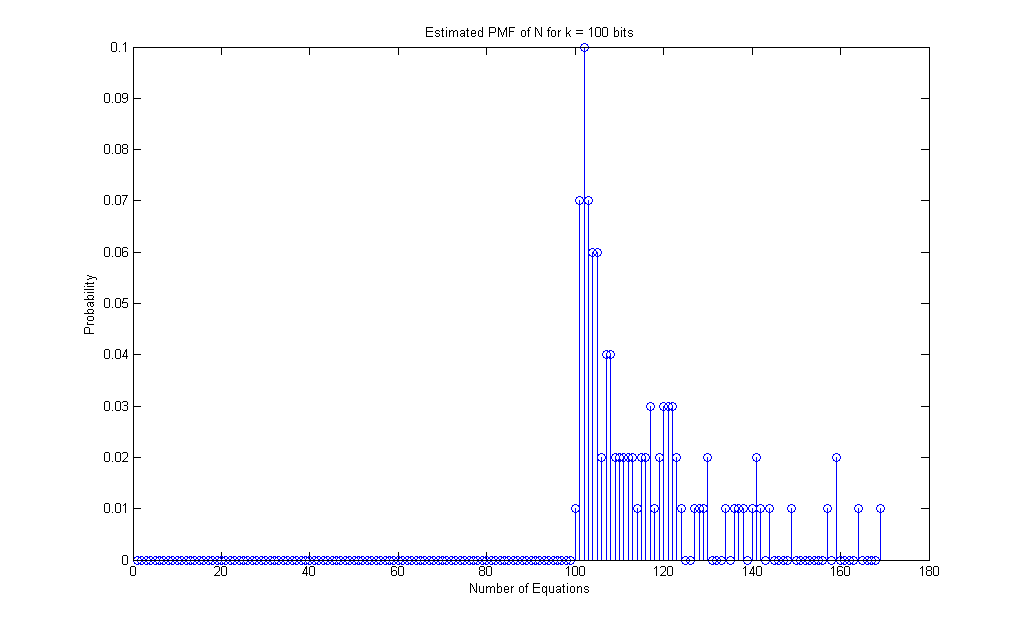
\includegraphics[width = 0.8\textwidth]{figure_1b_k100_ideal.png}
            \caption{Generic equation-solving with the Ideal Soliton degree distribution.}
        \end{center}
    \end{figure}

    \begin{figure}[H]
        \begin{center}
            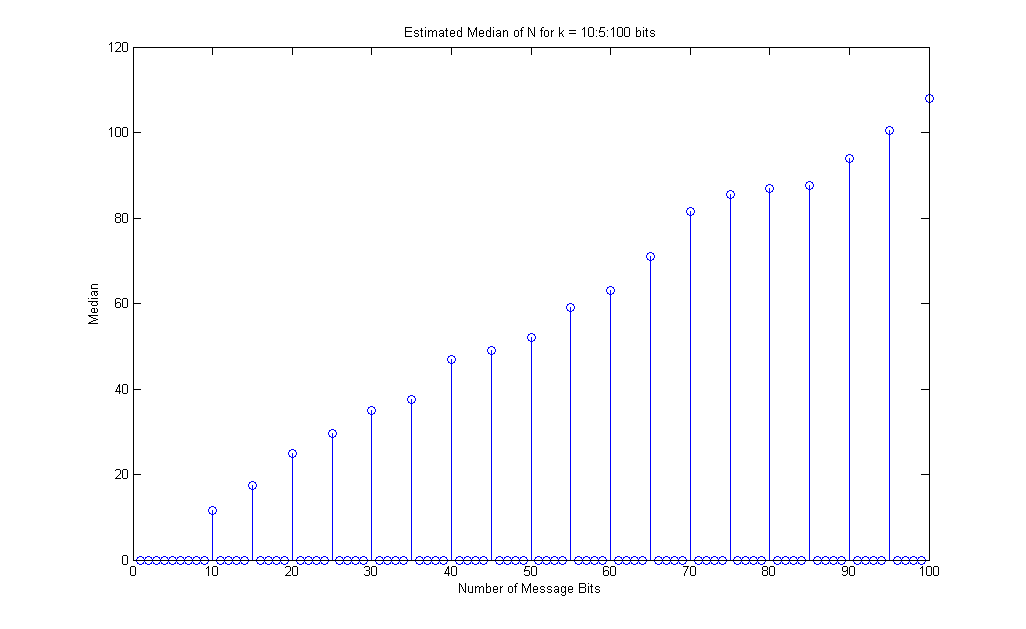
\includegraphics[width = 0.8\textwidth]{figure_1b_median_ideal.png}
            \caption{Generic equation-solving with the Ideal Soliton degree distribution.}
        \end{center}
    \end{figure}

    \begin{figure}[H]
        \begin{center}
            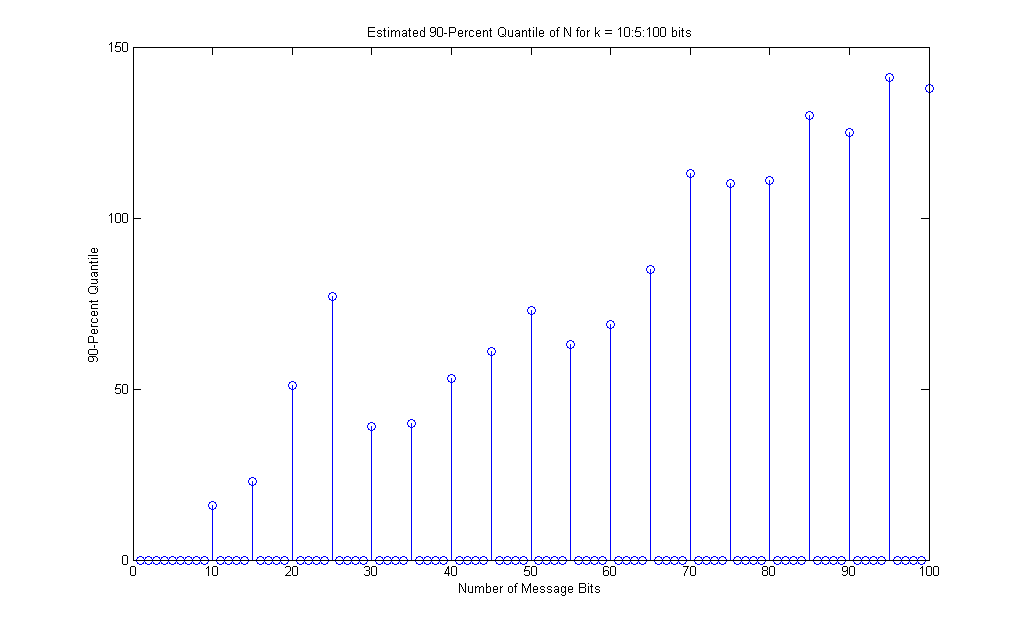
\includegraphics[width = 0.8\textwidth]{figure_1b_90_percent_quantile_ideal.png}
            \caption{Generic equation-solving with the Ideal Soliton degree distribution.}
        \end{center}
    \end{figure}

    \begin{figure}[H]
        \begin{center}
            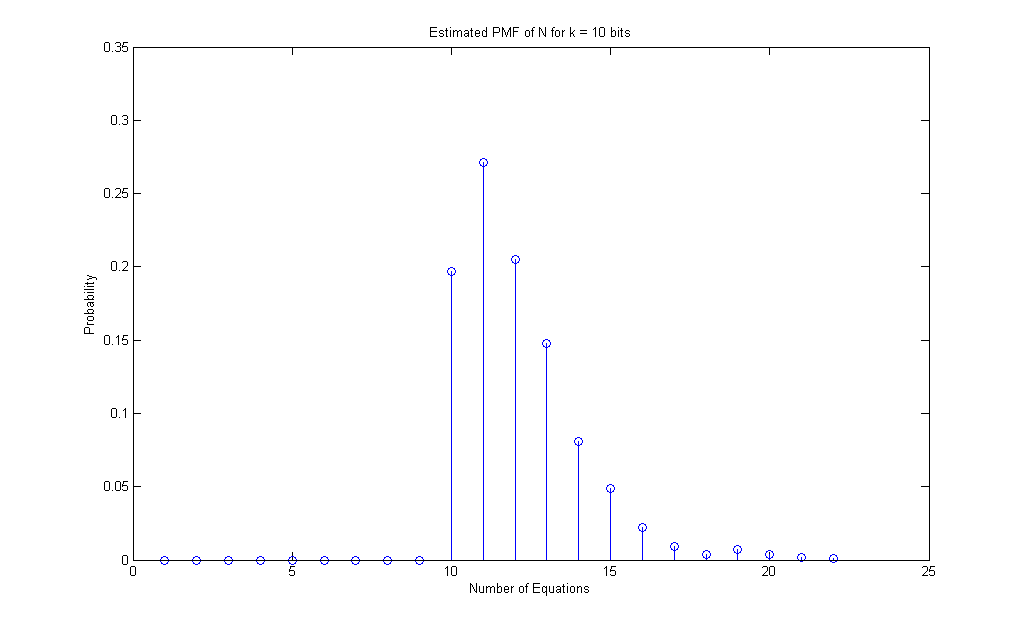
\includegraphics[width = 0.8\textwidth]{figure_1b_k10_robust.png}
            \caption{Generic equation-solving with the Robust Soliton degree distribution.}
        \end{center}
    \end{figure}

    \begin{figure}[H]
        \begin{center}
            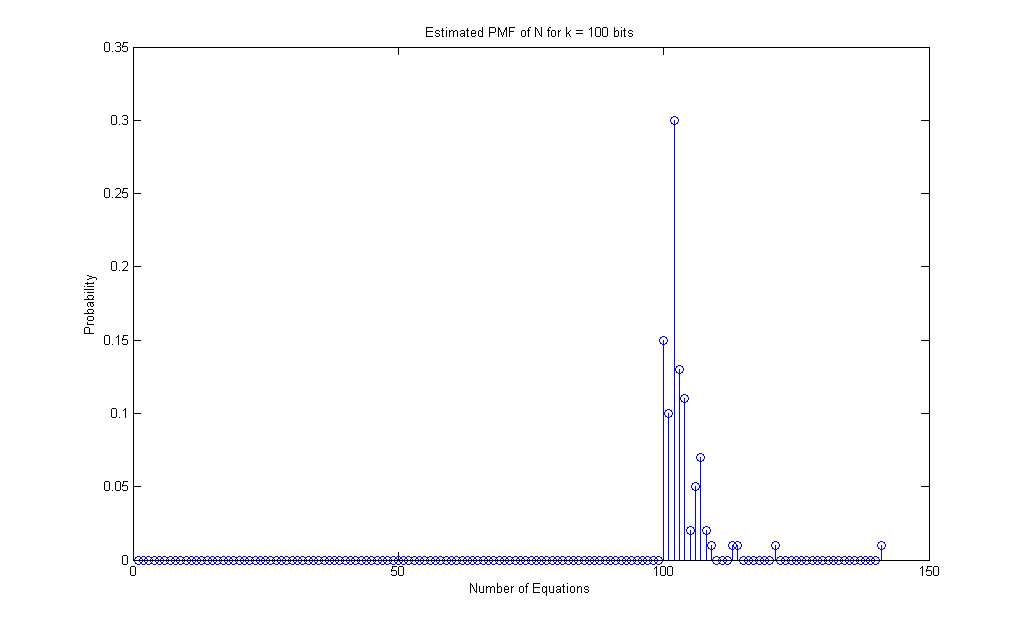
\includegraphics[width = 0.8\textwidth]{figure_1b_k100_robust.png}
            \caption{Generic equation-solving with the Robust Soliton degree distribution.}
        \end{center}
    \end{figure}

    \begin{figure}[H]
        \begin{center}
            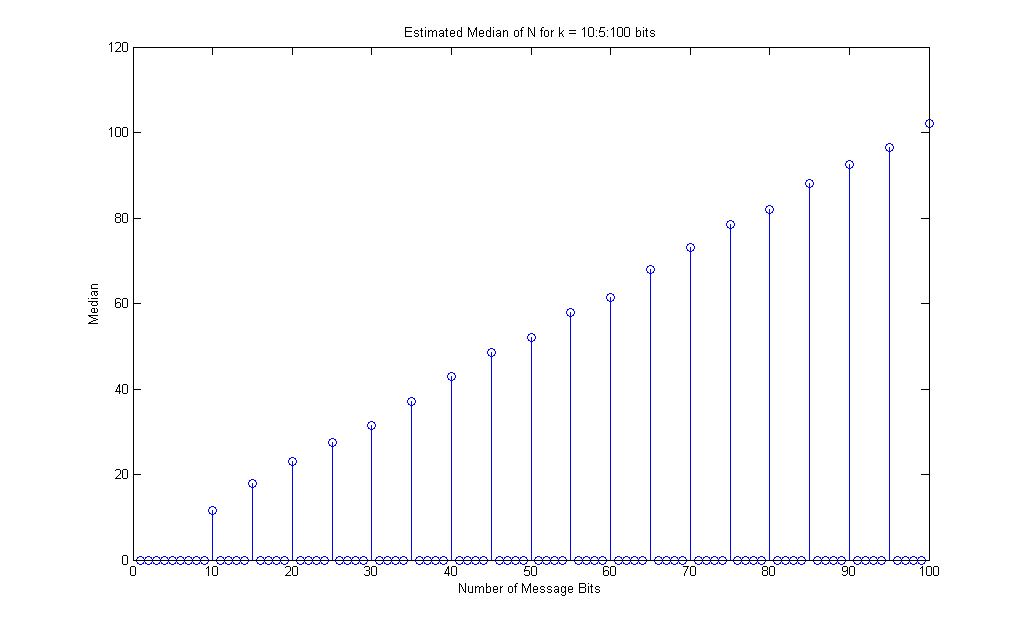
\includegraphics[width = 0.8\textwidth]{figure_1b_median_robust.png}
            \caption{Generic equation-solving with the Robust Soliton degree distribution.}
        \end{center}
    \end{figure}

    \begin{figure}[H]
        \begin{center}
            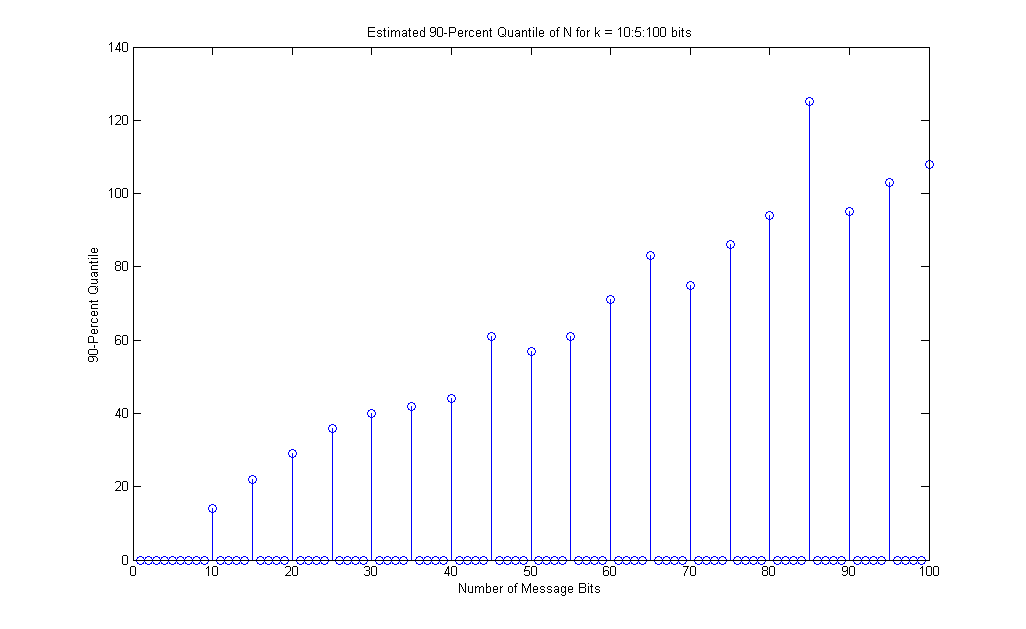
\includegraphics[width = 0.8\textwidth]{figure_1b_90_percent_quantile_robust.png}
            \caption{Generic equation-solving with the Robust Soliton degree distribution.}
        \end{center}
    \end{figure}

    \begin{figure}[H]
        \begin{center}
            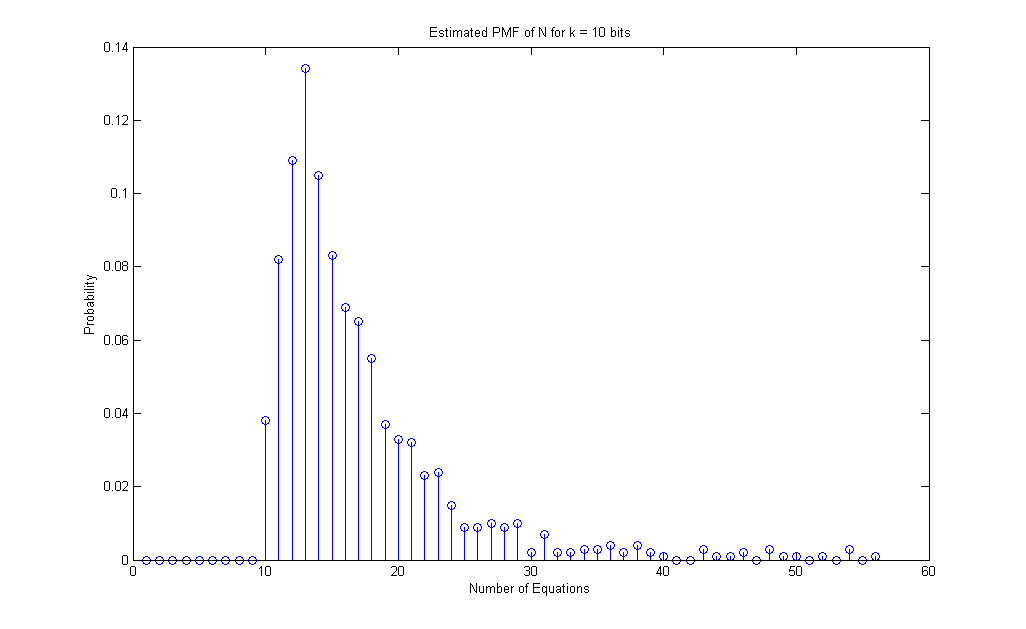
\includegraphics[width = 0.8\textwidth]{figure_1c_k10_ideal.png}
            \caption{Substitution-only-based equation-solving with the Ideal Soliton degree distribution.}
        \end{center}
    \end{figure}

    \begin{figure}[H]
        \begin{center}
            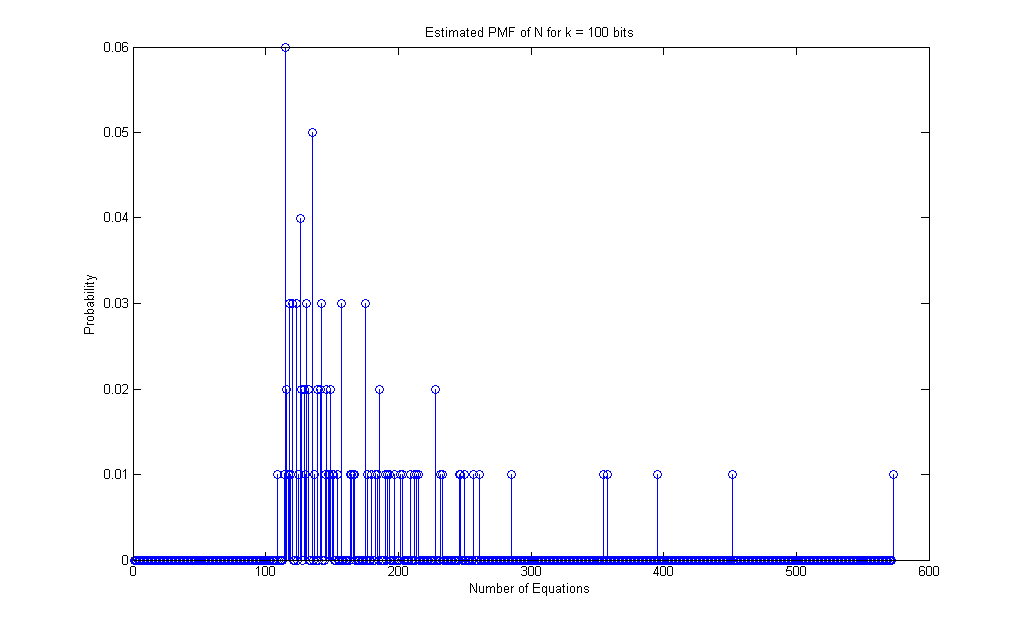
\includegraphics[width = 0.8\textwidth]{figure_1c_k100_ideal.png}
            \caption{Substitution-only-based equation-solving with the Ideal Soliton degree distribution.}
        \end{center}
    \end{figure}

    \begin{figure}[H]
        \begin{center}
            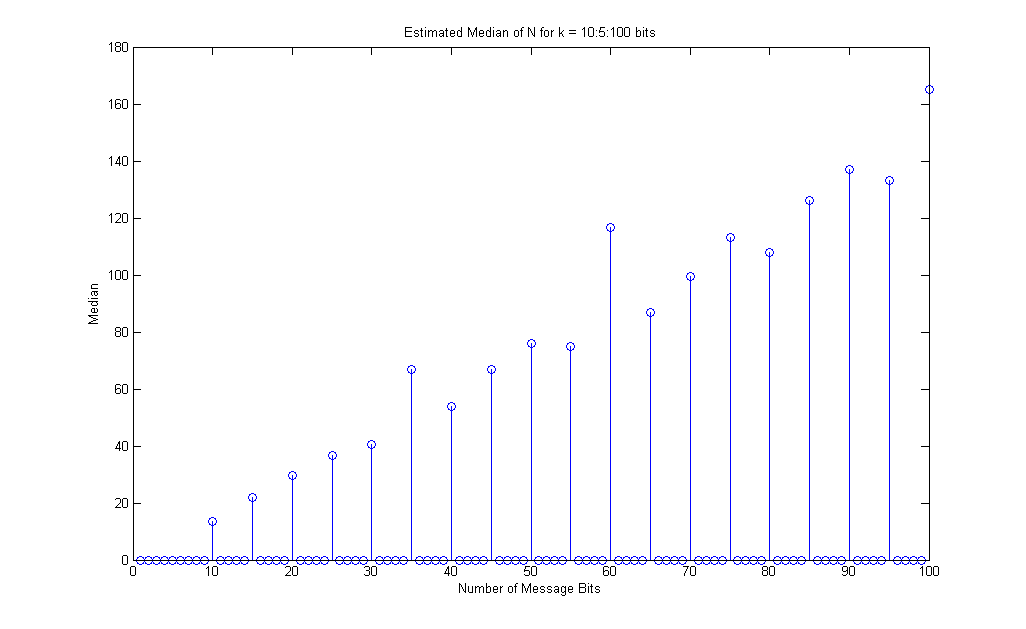
\includegraphics[width = 0.8\textwidth]{figure_1c_median_ideal.png}
            \caption{Substitution-only-based equation-solving with the Ideal Soliton degree distribution.}
        \end{center}
    \end{figure}

    \begin{figure}[H]
        \begin{center}
            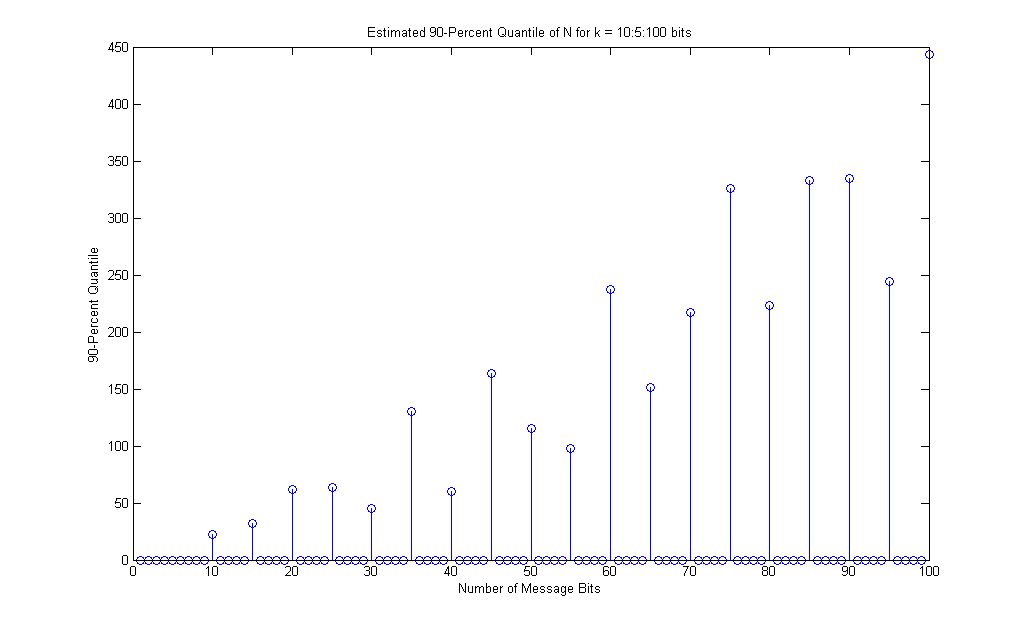
\includegraphics[width = 0.8\textwidth]{figure_1c_90_percent_quantile_ideal.png}
            \caption{Substitution-only-based equation-solving with the Ideal Soliton degree distribution.}
        \end{center}
    \end{figure}

    \begin{figure}[H]
        \begin{center}
            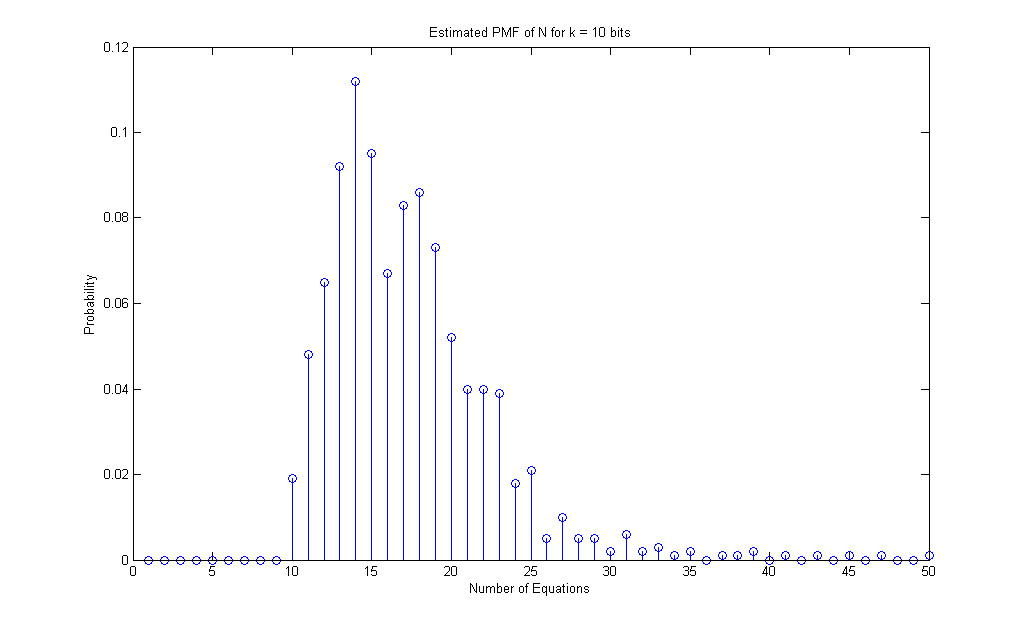
\includegraphics[width = 0.8\textwidth]{figure_1c_k10_robust.png}
            \caption{Substitution-only-based equation-solving with the Robust Soliton degree distribution.}
        \end{center}
    \end{figure}

    \begin{figure}[H]
        \begin{center}
            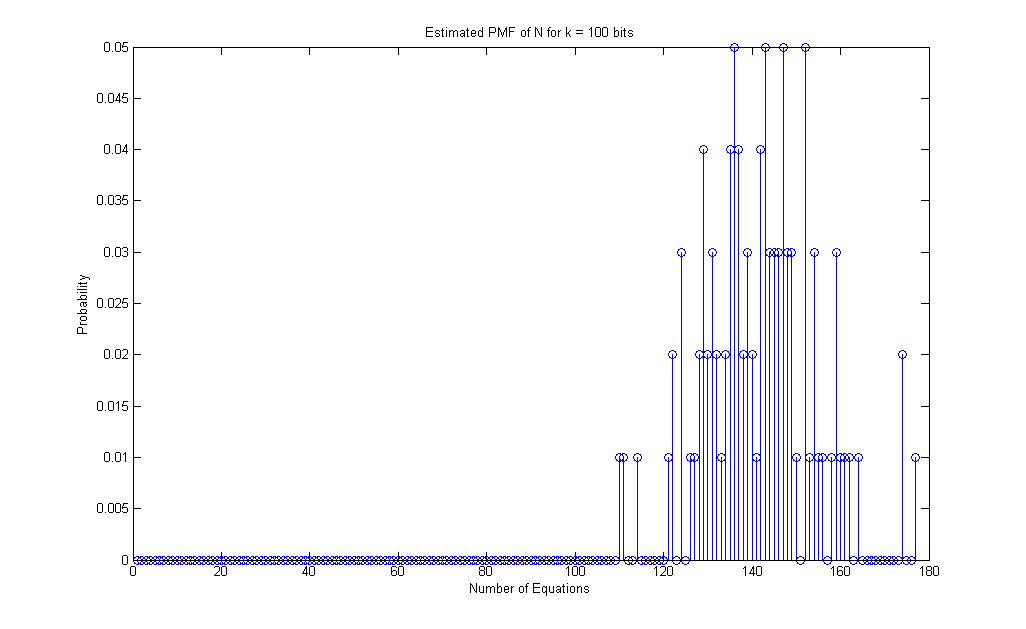
\includegraphics[width = 0.8\textwidth]{figure_1c_k100_robust.png}
            \caption{Substitution-only-based equation-solving with the Robust Soliton degree distribution.}
        \end{center}
    \end{figure}

    \begin{figure}[H]
        \begin{center}
            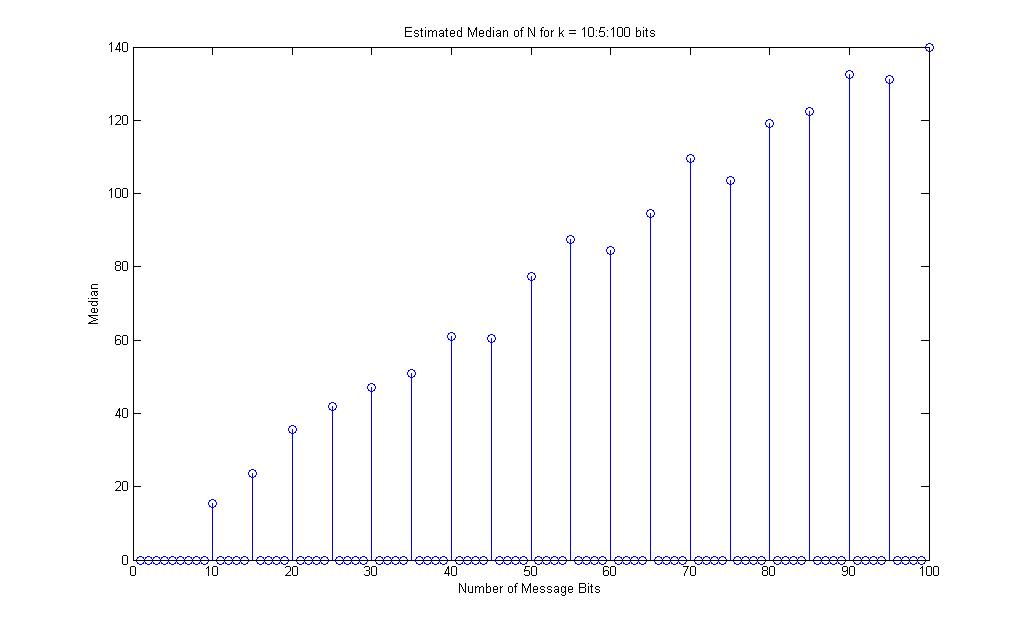
\includegraphics[width = 0.8\textwidth]{figure_1c_median_robust.png}
            \caption{Substitution-only-based equation-solving with the Robust Soliton degree distribution.}
        \end{center}
    \end{figure}

    \begin{figure}[H]
        \begin{center}
            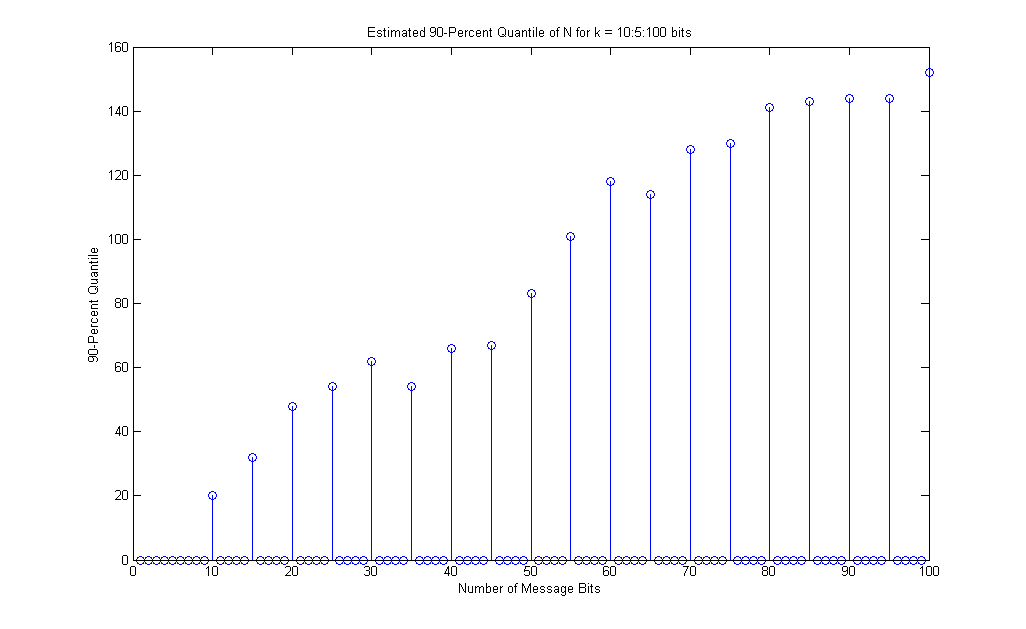
\includegraphics[width = 0.8\textwidth]{figure_1c_90_percent_quantile_robust.png}
            \caption{Substitution-only-based equation-solving with the Robust Soliton degree distribution.}
        \end{center}
    \end{figure}



    \newpage




% PROBLEM 2
  \item
    \begin{enumerate}

        % part a)
        \item Let $\vec{m} = [m_1 \cdots m_k]^\top$ be our message of length $k$. We will use a randomly generated ($\mathcal{B}(\frac{1}{2})$) parity check matrix H which will create an $s$-bit parity vector $\vec{p}$ such that
        \begin{equation*}
        \textbf{H}\vec{m} = \begin{bmatrix}
            p_1 \\
            \vdots\\
            p_s
            \end{bmatrix} = \vec{p}
        \end{equation*}

        where each $p_i$ checks the parity of the elements $m_j \in \vec{m}$ such that $H_{i,j} = 1$ where $j \in \{1, \cdots, k\}$. \newline

        If we assume our parity vector $\vec{p}$ can be transmitted error free, and that the number of parity bits $s = \vert \vec{p} \vert = \frac{k}{\alpha}$ where $\alpha > 1$, we can decode using a strategy similar to syndrome decoding.  There is a slight difference, however, in how our decoding strategy will work because we are guaranteed that the syndrome will go through without errors. Let us assume we sent the vector $[ \vec{m}^\top \vert \vec{p}^\top]^\top$ and we receive a noisy version $\vec{y}$. Then we can left multiply by $H$ to get
        \begin{equation*}
        H\vec{y} = H(\vec{x} + \vec{n}) = H\vec{x} + H\vec{n}
        \end{equation*}

        But we already know the value of $H\vec{x}$, so we can just subtract to get $H\vec{n}$. From this value we can determine the lowest weight noise value that would result in the syndrome $H\vec{n}$. The only source of error would be if two different low-weight noise vectors $\vec{n}$ and $\vec{n^*}$ would have the same syndrome $H\vec{n} = H\vec{n^*}$. We will show that this is unlikely by the AEP, given some bound on $\alpha$. We can see that the two syndromes $H\vec{n}$ and $H\vec{n^*}$ are marginally uniform because they are generated by a random generator matrix (if you really wanted to be more rigorous you could add an affine component to both and then just subtract it away after the analysis is done, but we trust that you can do this and don't mind our describing the syndromes and marginally uniform).

        By the AEP you can say, how many different noise vectors are there? $2^{k(H(p) + \epsilon)}$. How many different syndromes are there? $2^s$. What's the probability that a syndrome is also a noise vector? $\frac{2^{k(H(p) + \epsilon)}}{2^s} = \frac{2^{k(H(p) + \epsilon)}}{2^{k/\alpha}} = 2^{-k\times(\frac{1}{\alpha} - H(p) - \epsilon)}$ which goes to zero if $\alpha < \frac{1}{H(p) + \epsilon}$


        % part b)
        \item
            Let $\vec{m}$ be a $k = \alpha s$ bit message that we'd like to send over an unreliable erasure channel (BEC with bit-erasure probability $p$) without any coding, and assume we can send $\vec{r} = H\vec{m}$, the $s$-bit parity of $\vec{m}$, over a reliable channel (i.e. the receiver knows $\vec{r}$). The receiver also gets $\vec{y}$, which is the result of sending $\vec{m}$ over the BEC. Since all non-erased bits are correct, for each $y_i$ that is not erased, we have $y_i = m_i$. Our scheme works as follows:
            \begin{itemize}
                \item Compute $H\vec{y}$ and replace each erasure with some variable $e_i$.
                \item Were there no erasures, we would have $H\vec{y} = H\vec{m} = \vec{r}$. So, we set $H\vec{y} = \vec{r}$, yielding the following system of equations,
                    \begin{flalign*}
                        h_{11}y_1 + \dotsc + h_{1k}y_k &= r_1 \\
                        &\vdots \\
                        h_{s1}y_1 + \dotsc + h_{sk}y_k &= r_s
                    \end{flalign*}
                    where some number of the $y_i$s will be replaced with $e_i$s.
                \item Solve for all $e_i$s and reconstruct $\vec{m}$.
            \end{itemize}
            The Law of Large Numbers tells us we should expect roughly $k(p + \epsilon)$ erasures, so we decode only when less than $k(p + \epsilon)$ erasures occur, otherwise we declare error. If there aren't too many erasures, error occurs if any false message's syndrome (parity bits) matches the received message $\vec{y}$'s syndrome ($H\vec{y}$, with erasures) -- this occurs when a false message matches the received message (with erasures). We can compute the probability of error as follows:
            \begin{flalign*}
                P(\mbox{error}) &= P(\mbox{at least one false syndrome matches received syndrome}) \\
                &\leq 2^s\cdot2^{-k(p + \epsilon)} \\
                &= 2^{s - k(p + \epsilon)} \\
                &= 2^{s(1 - \alpha(p + \epsilon))}
            \end{flalign*}
            The inequality comes from a union bound -- there are $2^s$ possible syndromes, and the probability of any one false syndrome matching the received syndrome is equal to the probability that all of the non-erased message bits match a false message. There are $2^k$ total messages, and if we only decode when there are $k(1 - (p + \epsilon))$ non-erased bits, there are $2^{k(1 - (p + \epsilon))}$ messages that could match the received message with erasures. Then the probability of one false syndrome matching the received syndrome is simply $\frac{2^{k(1 - (p + \epsilon))}}{2^k} = 2^{-k(p + \epsilon)}$. \\
            \\
            We then choose the "reliability amplification" parameter $\alpha$ such that the probability of error goes to zero with $s$, i.e. the exponent in the probability of error must be negative:
            \begin{flalign*}
                1 - \alpha(p + \epsilon) &< 0 \\
                \alpha &> \frac{1}{p + \epsilon}
            \end{flalign*}
            And thus we see that, if we choose $\alpha > \frac{1}{p}$, this scheme will work with probability of error going to zero with $s$.

        % part c)
        \item
            Consider a message $\vec{m}$ of length $n = \alpha k = \alpha^2 s$. We would like to send this message over an unreliable channel without any coding. Let $H_1$ be a dense random parity-check matrix that linearly maps $n = \alpha k$ bits into $k$ parities. In parts a) and b), we showed that we can recover $\alpha s$ unreliable bits from $s$ reliable bits. So, if we can reliably send the $k$ parity bits computed via $H_1\vec{m}$, we can use them to recover the $n = \alpha k$ bits of $\vec{m}$. How do we reliably send the $k$ parity bits of $H_1\vec{m}$? We use the same strategy: let $H_2$ be a different dense random parity-check matrix that linearly maps $k = \alpha s$ bits into $s$ parities. We can then recover the $k = \alpha s$ bits of $H_1\vec{m}$ from the $s$ parity bits computed via $H_2(H_1\vec{m})$, since we can send $s$ bits reliably. Thus, if we can reliably send the $s$ bits of $H_2(H_1\vec{m})$, we can use them to recover the $k = \alpha s$ bits of $H_1\vec{m}$, which we can use to recover the $n = \alpha k = \alpha^2 s$ bits of $\vec{m}$.

        % part d)
        \item

        \begin{itemize}
            \item
                {\bf Binary Symmetric Channel} \\
                \\
                Let $\vec{t}$ be the $s$ bit message we're trying to communicate. We want to use a $\frac{1}{R}$-repetition code to encode $\vec{t}$ as $\vec{u}$, an $\frac{s}{R}$ bit codeword made up of $s$ blocks, each containing $\frac{1}{R}$ bits. We then send $\vec{u}$ over a BSC with bit-error probability $p$. Call the received codeword (with errors) $\vec{v}$. We decode $\vec{v}$ to the $s$ big message $\hat{t}$ via majority decoding:
                \begin{itemize}
                    \item
                        For the $i^{\mbox{th}}$ block of $\vec{v}$:
                            \begin{itemize}
                                \item
                                    If there are more ones than zeros, decode the $i^{\mbox{th}}$ bit of $\hat{t}$ as one, and vice versa.
                            \end{itemize}
                \end{itemize}
                In this scheme, an error occurs if at least half of the bits in at least one block are corrupt. For a single block, let $X_i$ be an indicator random variable on the $i^{\mbox{th}}$ bit in the block being corrupt ($X_i\sim\mathcal{B}(p)$, i.i.d. over $i$), and let $Y = \sum_{i = 1}^{\frac{1}{R}}$. Then:
                \begin{flalign*}
                    P(\mbox{at least half of one block is corrupt}) &= P(Y \geq \frac{1}{2}\cdot\frac{1}{R}) \\
                    &\leq \underset{t > 0}{\mbox{min}} \frac{\prod_{i = 1}^{\frac{1}{R}}\mathbb{E}[e^{tX_i}]}{e^{\frac{t}{2R}}}
                \end{flalign*}
                The above inequality is the result of a Chernoff bound. It can be shown that, for a sum of i.i.d. $\mathcal{B}(p)$ random variables, the minimizing $t$ is $\log{\frac{1 - p}{p}}$. Substituting this value yields:
                \begin{flalign*}
                    P(\mbox{block error}) &\leq (2(p(1 - p))^{\frac{1}{2}})^{\frac{1}{R}} \\
                    P(\mbox{error}) &= P(\mbox{at least one block error}) \leq s\cdot(2(p(1 - p))^{\frac{1}{2}})^{\frac{1}{R}}
                \end{flalign*}
                The last equality is the result of a union bound -- all bit-erasures are independent, so all block-erasures are independent. If we are willing to tolerate $P(\mbox{error}) \leq \delta$, then:
                \begin{flalign*}
                    P(\mbox{error}) \leq s\cdot(2(p(1 - p))^{\frac{1}{2}})^{\frac{1}{R}} &\leq \delta \\
                    \frac{1}{R}\log{(2(p(1-p))^{\frac{1}{2}})} \leq \log{\frac{\delta}{s}} \\
                    \frac{1}{R} \geq \frac{\log{\frac{\delta}{s}}}{\log{(2(p(1 - p))^{\frac{1}{2}})}}
                \end{flalign*}
                Thus, if we repeat each bit of $\vec{t}$ at least $\frac{\log{\frac{\delta}{s}}}{\log{(2(p(1 - p))^{\frac{1}{2}})}}$ times, we will successfully communicate $\vec{t}$ with probability $1 - \delta$. The rate of this code is then $R \leq \frac{\log{(2(p(1 - p))^{\frac{1}{2}})}}{\log{\frac{\delta}{s}}}$

            \item
                {\bf Binary Erasure Channel} \\
                \\
                Let $\vec{t}$ be the $s$ bit message we're trying to communicate. We want to use a $\frac{1}{R}$-repetition code to encode $\vec{t}$ as $\vec{u}$, an $\frac{s}{R}$ bit codeword made up of $s$ blocks, each containing $\frac{1}{R}$ bits. We then send $\vec{u}$ over a BEC with bit-erasure probability $p$. Call the received codeword (with erasures) $\vec{v}$. Since all non-erased bits are correct, we decode $\vec{v}$ to the $s$ bit message $\hat{t}$ via the following strategy:
                \begin{itemize}
                    \item
                        For the $i^{\mbox{th}}$ block of $\vec{v}$:
                            \begin{itemize}
                                \item
                                    If not all bits are erased, decode bit $i$ of $\hat{t}$ as the non-erased bits of block $i$.
                            \end{itemize}
                \end{itemize}
                In this scheme, an error occurs if at least one block has all $\frac{1}{R}$ bits erased.
                \begin{flalign*}
                P(\mbox{all bits in one block erased}) &= p^{\frac{1}{R}} \\
                P(\mbox{error}) &= P(\mbox{all bits in at least one block erased}) \leq s\cdot p^{\frac{1}{R}}
                \end{flalign*}
                The last equality is the result of a union bound -- all bit-erasures are independent, so all block-erasures are independent. If we are willing to tolerate $P(\mbox{error}) \leq \delta$, then:
                \begin{flalign*}
                    P(\mbox{error}) \leq s\cdot p^{\frac{1}{R}} &\leq \delta \\
                    p^{\frac{1}{R}} &\leq \frac{\delta}{s} \\
                    \log{p^{\frac{1}{R}}} \leq \log{\frac{\delta}{s}} \\
                    \frac{1}{R}\log{p} \leq \log{\frac{\delta}{s}} \\
                    \frac{1}{R} \geq \frac{\log{\frac{\delta}{s}}}{\log{p}}
                \end{flalign*}
                Thus, if we repeat each bit of $\vec{t}$ at least $\frac{\log{\frac{\delta}{s}}}{\log{p}}$ times, we will successfully communicate $\vec{t}$ with probability $1 - \delta$. The rate of this code is then $R \leq \frac{\log{p}}{\log{\frac{\delta}{s}}}$
        \end{itemize}



        % part e)
        \item

        \begin{itemize}
            \item
                {\bf Binary Symmetric Channel} \\
                \\
                In part (a), we determined that we could find a suitable $\alpha$ such that the probability of error due to syndrome collisions goes to zero. Now, we extrapolate the scheme from (c) and (d) as follows:
                \begin{itemize}
                    \item Determine the number of stages $k$ via $n = \alpha^k s$, for some $s$.
                    \item Compute syndromes of syndromes of the $n$-bit message ($k$ times) until we have an $s$ bit parity that we will send reliably using an $m$-repetition code.
                    \item Use the $s$ parity bits to recover $\alpha s$ bits, which will be used to recover $\alpha^2 s$ bits, and so on, until we recover the $\alpha^{k - 1} s$-bit syndrome of the $n$-bit message, which we can use to recover the un-encoded $n = \alpha^k s$-bit message.
                \end{itemize}
                Since we can choose $\alpha$ such that the probability of error due to syndrome collisions goes to zero, of error occurs in the overall scheme if:
                \begin{itemize}
                    \item The repetition code fails, or:
                    \item The repetition code succeeds, but the noise corrupts the $\alpha s$-bit syndrome beyond recovery, or:
                    \item $\dotsc$
                    \item Everything up to and including the $\alpha^{k - 1} s$ bit syndrome succeeds, but the $n = \alpha^k s$-bit message is corrupted beyond recovery.
                \end{itemize}
                In part (d), we found the probability of the repetition code failing. Similarly, we can use a Chernoff bound to find the probability that the $j^{\mbox{th}}$ stage fails (when the noise behaves too weirdly, i.e. more than $\sim kp$ errors occur). Let $X_i$ be an indicator random variable on the $i^{\mbox{th}}$ bit in the $\alpha^j s$ bits being corrupt ($X_i\sim\mathcal{B}(p)$, i.i.d. over $i$), and let $Y = \sum_{i = 1}^{\alpha^j s}$. Then:
                \begin{flalign*}
                    P(\mbox{stage $j$ fails}) &= P(\mbox{noise behaves too weirdly}) \\
                    &= P(Y > \alpha^j sp) \\
                    &\leq (2(1 - p)^{1 - p}p^p)^{\alpha^j s}
                \end{flalign*}
                We use a union bound to estimate the block error, which we'd like to bound by $\delta$:
                \begin{flalign*}
                    P(\mbox{block error}) &= P(\mbox{any stage fails}) \\
                    &\leq P(\mbox{repetition code fails}) + P(\mbox{stage 1 fails}) + \dotsc + P(\mbox{stage $k$ fails}) \\
                    &= s\cdot(2(p(1 - p))^{\frac{1}{2}})^{m} + \sum_{j = 1}^{k} (2(1 - p)^{1 - p}p^p)^{\alpha^j s} < \delta
                \end{flalign*}
                If we've chosen a suitable $\alpha$, then all we need to do is find a long enough $m$ such that the block error is less than $\delta$:
                \begin{flalign*}
                    s\cdot(2(p(1 - p))^{\frac{1}{2}})^{m} + \sum_{j = 1}^{k} (2(1 - p)^{1 - p}p^p)^{\alpha^j s} &< \delta \\
                    s\cdot(2(p(1 - p))^{\frac{1}{2}})^{m} &< \delta - \sum_{j = 1}^{k} (2(1 - p)^{1 - p}p^p)^{\alpha^j s} \\
                    m\log{(2(p(1 - p))^{\frac{1}{2}})} &< \log{\frac{\delta - \sum_{j = 1}^{k} (2(1 - p)^{1 - p}p^p)^{\alpha^j s}}{s}} \\
                    m &> \frac{\log{\frac{\delta - \sum_{j = 1}^{k} (2(1 - p)^{1 - p}p^p)^{\alpha^j s}}{s}}}{\log{(\frac{1}{2}(p(1 - p))^{-\frac{1}{2}})}}
                \end{flalign*}
                Note that we have not specified any size for $s$. We could do so by choosing $s$ that minimizes $m$, while still keeping the block error probability bounded by $\delta$ -- this would maximize the overall rate $R$ of the code:
                \begin{flalign*}
                    R &= \frac{\mbox{message bits}}{\mbox{code bits}} \\
                    &= \frac{\alpha^k s}{ms + \sum_{j = 1}^k \alpha^j s} \\
                    &= \frac{\alpha^k}{m + \sum_{j = 1}^k \alpha^j}
                \end{flalign*}
                 Recall that the number of stages $k$ is determined by $n$, $\alpha$, and $s$, which we have now fixed. Thus we have a scheme in which everything is determined by the desired block error $\delta$. Additionally, we can make some approximations to simplify the expression for the rate. Since $n$ is large, $k$ will also be large, and $\alpha$ is greater than one, so we have:
                \begin{flalign*}
                    R &= \frac{\alpha^k}{m + \sum_{j = 1}^k \alpha^j} \\
                    &\approx \frac{\alpha^k}{\sum_{j = 1}^k \alpha^j} \\
                    &= \frac{\alpha^k}{\left(\frac{1 - \alpha^{k + 1}}{1 - \alpha} - 1\right)} \\
                    &\approx \frac{\alpha^k}{\frac{-\alpha^{k + 1}}{1 - \alpha}} \\
                    &= \frac{\alpha^k - \alpha^{k + 1}}{-\alpha^{k + 1}} \\
                    &= 1 - \frac{1}{\alpha}
                \end{flalign*}
            \item
                {\bf Binary Erasure Channel} \\
                \\
                In part (b), we determined that we could find a suitable $\alpha$ such that the probability of error due to syndrome collisions goes to zero. Now, we extrapolate the scheme from (c) and (d) as follows:
                \begin{itemize}
                    \item Determine the number of stages $k$ via $n = \alpha^k s$, for some $s$.
                    \item Compute syndromes of syndromes of the $n$-bit message ($k$ times) until we have an $s$ bit parity that we will send reliably using an $m$-repetition code.
                    \item Use the $s$ parity bits to recover $\alpha s$ bits, which will be used to recover $\alpha^2 s$ bits, and so on, until we recover the $\alpha^{k - 1} s$-bit syndrome of the $n$-bit message, which we can use to recover the un-encoded $n = \alpha^k s$-bit message.
                \end{itemize}
                Since we can choose $\alpha$ such that the probability of error due to syndrome collisions goes to zero, of error occurs in the overall scheme if:
                \begin{itemize}
                    \item The repetition code fails, or:
                    \item The repetition code succeeds, but the $\alpha s$-bit syndrome is erased beyond recovery, or:
                    \item $\dotsc$
                    \item Everything up to and including the $\alpha^{k - 1} s$ bit syndrome succeeds, but the $n = \alpha^k s$-bit message is erased beyond recovery.
                \end{itemize}
                In part (d), we found the probability of the repetition code failing. Similarly, we can use a Chernoff bound to find the probability that the $j^{\mbox{th}}$ stage fails (when the noise behaves too weirdly, i.e. more than $\sim kp$ erasures occur). Let $X_i$ be an indicator random variable on the $i^{\mbox{th}}$ bit in the $\alpha^j s$ bits being erased ($X_i\sim\mathcal{B}(p)$, i.i.d. over $i$), and let $Y = \sum_{i = 1}^{\alpha^j s}$. Then:
                \begin{flalign*}
                    P(\mbox{stage $j$ fails}) &= P(\mbox{noise behaves too weirdly}) \\
                    &= P(Y > \alpha^j sp) \\
                    &\leq (2(1 - p)^{1 - p}p^p)^{\alpha^j s}
                \end{flalign*}
                We use a union bound to estimate the block error, which we'd like to bound by $\delta$:
                \begin{flalign*}
                    P(\mbox{block error}) &= P(\mbox{any stage fails}) \\
                    &\leq P(\mbox{repetition code fails}) + P(\mbox{stage 1 fails}) + \dotsc + P(\mbox{stage $k$ fails}) \\
                    &= s\cdot p^{m} + \sum_{j = 1}^{k} (2(1 - p)^{1 - p}p^p)^{\alpha^j s} < \delta
                \end{flalign*}
                If we've chosen a suitable $\alpha$, then all we need to do is find a long enough $m$ such that the block error is less than $\delta$:
                \begin{flalign*}
                    s\cdot p^{m} + \sum_{j = 1}^{k} (2(1 - p)^{1 - p}p^p)^{\alpha^j s} &< \delta \\
                    s\cdot p^{m} &< \delta - \sum_{j = 1}^{k} (2(1 - p)^{1 - p}p^p)^{\alpha^j s} \\
                    m\log{p} &< \log{\frac{\delta - \sum_{j = 1}^{k} (2(1 - p)^{1 - p}p^p)^{\alpha^j s}}{s}} \\
                    m &> \frac{\log{\frac{\delta - \sum_{j = 1}^{k} (2(1 - p)^{1 - p}p^p)^{\alpha^j s}}{s}}}{\log{\frac{1}{p}}}
                \end{flalign*}
                Note that we have not specified any size for $s$. We could do so by choosing $s$ that minimizes $m$, while still keeping the block error probability bounded by $\delta$ -- this would maximize the overall rate $R$ of the code:
                \begin{flalign*}
                    R &= \frac{\mbox{message bits}}{\mbox{code bits}} \\
                    &= \frac{\alpha^k s}{ms + \sum_{j = 1}^k \alpha^j s} \\
                    &= \frac{\alpha^k}{m + \sum_{j = 1}^k \alpha^j} \\
                    &\approx 1 - \frac{1}{\alpha}
                \end{flalign*}
                Recall that the number of stages $k$ is determined by $n$, $\alpha$, and $s$, which we have now fixed. Thus we have a scheme in which everything is determined by the desired block error $\delta$.


        \end{itemize}


        %part f)
        \item
        	Assuming that we have $k$ message bits and some of them are erased and $s$ bits of message syndrome that are transmitted perfectly, we construct a graph where each of the $k$ message bits are directly connected to nodes at their corresponding index in the message we are trying to decode. The syndrome bits are connected to the nodes of the message we are trying to decode by drawing an edge to each index that was involved in the XOR that created that parity bit. When we decode, the received message bits that were not erased are pushed up to our decoded message nodes. We then attempt to use the edges with the parity bits to push bits to the decoded message slots that we don't have. There are times when we get stuck with this strategy. If we are unlucky with the combination of our parity check matrix and our erasures we can get in a situation where we lack enough information to come up with a unique solution for the decoded message. \\
	\begin{center}
	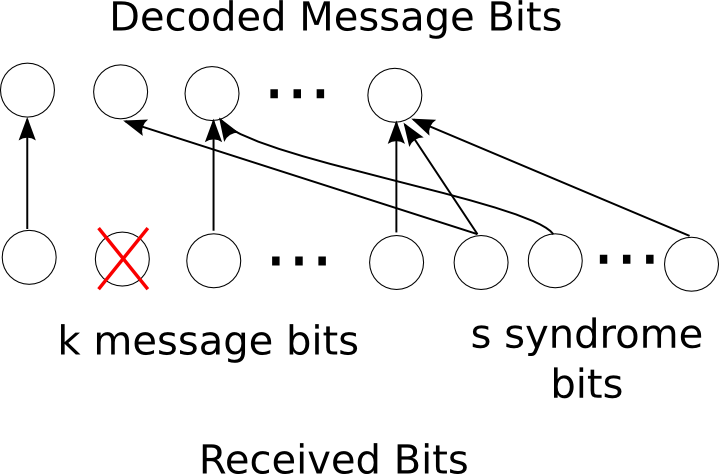
\includegraphics[scale=0.5, angle=0]{../hw3-f.png}
	\end{center}


        %part g)
        \item
            If we use a parity matrix $H$ with exactly three ones in each column and exactly thirty ones in each row, this means the bipartite graph representation has $3k$ edges going from the $k$ data bits to the $s$ parity bits and $30s$ edges going from the $s$ parity bits to the $k$ data bits. Both numbers must be the same, so we set them equal to each other and solve:
            \begin{flalign*}
                30s = 3k \\
                s = \frac{k}{10}
            \end{flalign*}
            So, for $k$ data bits, there are $\frac{k}{10}$ parity bits, and the size of $H$ is $\frac{k}{10} \times k$ (rows $\times$ columns).


        %part h)
        \item
            We will find the probability that a loop exists in the first level of the tree by drawing a parallel between this problem and the Birthday Paradox. There are $k$ total data bits in the tree, and there are 88 data bits in the first level. A cycle exists if any data bit shows up more than once in the first level. Let us look at the total number of data bits $k$ as the total number of possible birthdays, and the 88 data bits as the number of people in a room. The probability of a loop existing is the complement of the probability that no loop exists, which is equivalent to the probability that no data bit shows up more than once, which is equivalent to no two people of the 88 people in a room having the same birthday. This probability is:
            \begin{flalign*}
                P(\mbox{no two people have the same birthday}) &= \frac{k\mbox{P}88}{k^{88}} \\
                &= \frac{k!}{(k - 88)!k^{88}} \\
                &= \frac{(k - 0)(k - 1)\cdots(k - 87)}{k^{88}} \\
                &= \frac{k^{88}}{k^{88}}(1 - \frac{0}{k})(1 - \frac{1}{k})\dotsc(1 - \frac{86}{k}) \\
                &\approx 1 - e^{-\frac{0}{k}}e^{-\frac{1}{k}}\dotsc e^{-\frac{87}{k}} \\
                &= e^{-\frac{1}{k}\sum_{i = 1}^{87}} \\
                &= e^{-\frac{87\cdot86}{2k}}
            \end{flalign*}
            The probability of a loop existing in the first level is simply the complement of the above probability, and we want to bound that by $\delta$:
            \begin{flalign*}
                1 - e^{-\frac{87\cdot86}{2k}} &\leq \delta \\
                e^{-\frac{87\cdot86}{2k}} &\geq 1 - \delta \\
                -\frac{87\cdot86}{2k} &\geq \log{1 - \delta} \\
                k &\geq \frac{87\cdot86}{\log{\frac{1}{1 - \delta}}}
            \end{flalign*}
            Thus, if we are willing to tolerate a loop probability of $\delta$, $k$ must be larger than $\frac{87\cdot86}{\log{\frac{1}{1 - \delta}}}$.


        % part i)
        \item
        	If we look at the tree after the zero-th level (1 data node with the 3 parity nodes) there are an additional 29 data nodes with 2 parity nodes extending from them. We can therefore describe the number of data and parity nodes with the following pattern: \\
	\begin{eqnarray*}
	D_0=1 \\ P_0=3 \\ P_{-1}=0 \\
	D_i=29(P_{i-1}-P_{i-2})+D_{i-1} \\
	P_i=2(D_i-D_{i-1})+P_{i-1} \\
	\end{eqnarray*}
	We then look at this problem in the same way as the previous one except now we are looking at the chance that a data node or a parity node occurs more than once. So first let's find the probability that there are no repeated data or parity nodes at a depth of $i$. \\
	\begin{eqnarray*}
	   P(\mbox{no two data nodes are the same}) = \frac{k\mbox{P}D_i}{k^{D_i}} = \frac{k!}{(k-D_i)!k^{D_i}}\\
	   P(\mbox{no two parity nodes are the same}) = \frac{\frac{k}{10}\mbox{P}P_i}{\frac{k}{10}^{P_i}} = \frac{\frac{k}{10}!}{(\frac{k}{10}-P_i)!\frac{k}{10}^{P_i}}\\
	   P(\mbox{no two nodes are the same}) = \left(\frac{k!}{(k-D_i)!k^{D_i}}\right)\left(\frac{\frac{k}{10}!}{(\frac{k}{10}-P_i)!\frac{k}{10}^{P_i}}\right) \\
	   P(\mbox{no loops at depth i}) = 1- \left(\frac{k!}{(k-D_i)!k^{D_i}}\right)\left(\frac{\frac{k}{10}!}{(\frac{k}{10}-P_i)!\frac{k}{10}^{P_i}}\right) \leq \delta \\
	\end{eqnarray*}
	
	Using similar analysis as the problem above we jump to the following approximation and solve for the bound on k: \\
	\begin{eqnarray*}
	   1-\left(e^{\frac{-(D_i-1)(D_i-2)}{2k}}\right)\left(e^{\frac{-(P_i-1)(P_i-2)}{2\frac{k}{10}}}\right) \leq \delta \\
	   1- \delta \leq e^{\frac{-(D_i-1)(D_i-2)-10(P_i-1)(P_i-2)}{2k}} \\
	   ln(1-\delta) \leq \frac{-(D_i-1)(D_i-2)-10(P_i-1)(P_i-2)}{2k} \\
	   k \geq \frac{(D_i-1)(D_i-2)+10(P_i-1)(P_i-2)}{2 \log{\frac{1}{1-\delta}}} \\
	\end{eqnarray*}
	Solving the above recurrence relations yields:
        \begin{flalign*}
            D_i &= \frac{1}{19}(29\cdot58^i - 10) \\
            P_i &= \frac{1}{19}(58^i - 1)
        \end{flalign*}
    Substituting, we have:
    \begin{flalign*}
        k &\geq \frac{1}{361}(-2823\cdot58^i + 851\cdot3364^i + 9192)
    \end{flalign*}

        % part j)
        \item
            An erased bit at level $i - 1$ is unable to be recovered if both of its lower-neighbor parity bits are useless. A parity bit is useless if it is erased, or if any of its 29 lower-neighbor data bits are erased, since we decode by pushing/XORing lower-neighbor data bits up into parity bits. Since we are assuming the $s$ parity bits were sent reliably, we will just worry about the case where any of a parity bit's lower-neighbor data bits are erased. The probability of a data bit being erased is $p$, and the probability that any of a parity bit's lower-neighbor data bits are erased is $1 - (1 - p)^29$. A data bit has two lower-neighbor parity bits, so we have:
            \begin{flalign*}
                p_e[i - 1] &= p(1 - (1 - p)^{29})^2
            \end{flalign*}
            Generalizing, we have:
            \begin{flalign*}
                p_e[j - 1] &= p(1 - (1 - p_e[j])^{29})^2
            \end{flalign*}
            For $j = 1$, the root data bit has three lower-neighbor parity bits, so we have:
            \begin{flalign*}
                p_e[0] &= p(1 - (1 - p_e[1])^{29})^3
            \end{flalign*}

        % part k)
        \item
            In part j we found $f(x) = (1 - (1 - x)^{29})^2$. From the plot, we see that, for $p = 0.05$, the path taken by the probability of error on a bit as we move up the tree towards the root converges to zero:
        \begin{figure}[H]
            \begin{center}
                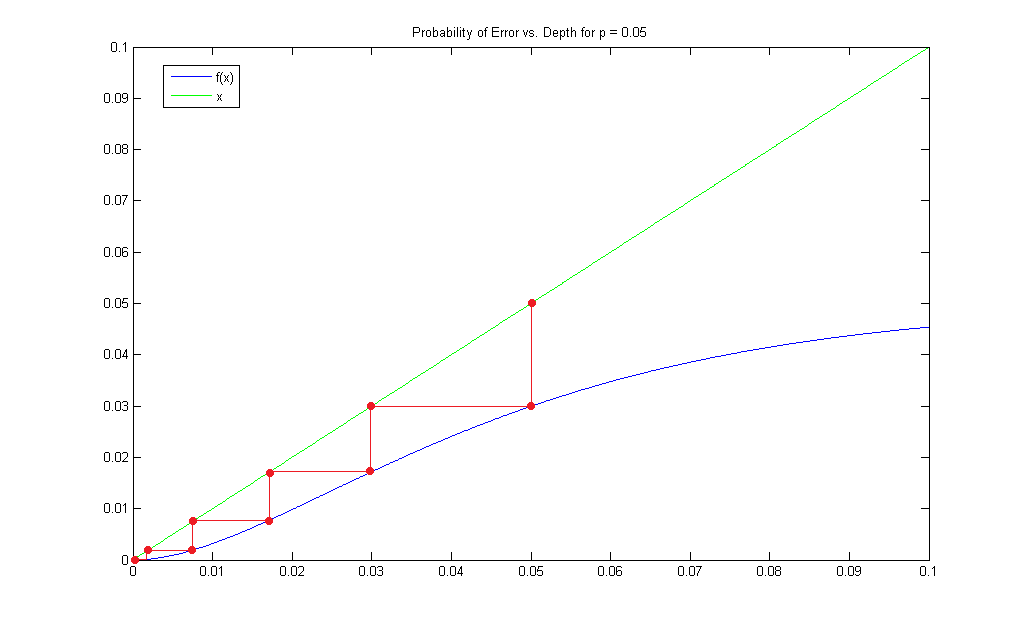
\includegraphics[width = \textwidth]{figure_k.png}
                \caption{}
            \end{center}
        \end{figure}


        % part l)
        \item
            Taylor expanding $f(x)$ in the neighborhood of $x = 0$ yields:
            \begin{flalign*}
                f(x) &\approx 841px^2 - 23548px^3 + O(x^4)
            \end{flalign*}
            Since $x$ (the probability of that a lower-level bit is both erased and unable to be recovered) is very small (much less than one), the first term dominates: $f(x) \approx 841px^2$. Since $p$ is also less than one, $841px^2$ should be less than one. After $m$ iterations of the decoding process, we have something like $f(f(\dotsc f(x))) \approx (\alpha x^2)^{2m}$, where $\alpha$ is less than one. Thus we see the probability of error is converging to zero quite fast, like something less than one to the $2m^{\mbox{th}}$ power.

        % part m)
        \item

        % part n)
        \item
            By increasing $p$ and re-plotting until $f(x)$ intersects the function $x$, we see that the decoding method will fail roughly around $p \geq 0.083$:
        \begin{figure}[H]
            \begin{center}
                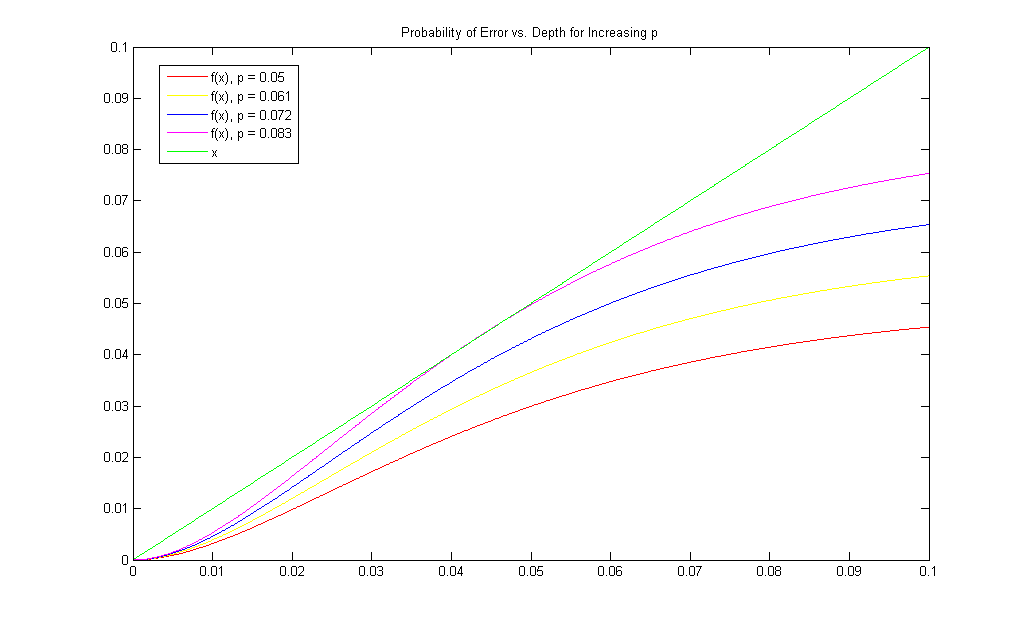
\includegraphics[width = \textwidth]{figure_n.png}
                \caption{}
            \end{center}
        \end{figure}
            \noindent
        % part o)
        \item
            From the plot in the previous part, we see that, from about $p = 0.03$ to $p = 0.05$, $f(x)$ is very close to the function $x$. This means the path taken by the probability of error has a lot more "turns" than it would for lower values of $p$. In other words, since $f(x)$ and the function $x$ are very close for values of $p$ close to the threshold value, the path "bounces" back \& forth very rapidly, which means the decoding process will take many, many more iterations.


        % part p)
        \item




    \end{enumerate}
    \newpage



  % PROBLEM 3
  \item
  {\bf Question:} 
        EXIT charts are a tool for the analysis of iteratively decoded error-correcting codes. In an EXIT-like chart (from question 2), explain qualitatively the consequences of increasing the probability of error p. What happens graphically? How does this relate to the actual iterative decoding?
        
        
        
    {\bf Answer:}
    	As seen in figures 21 and 22, the higher the probability of error is, the higher the function f(x) is, closer to the curve y=x. Starting the iteration from the specific p shows the stair-step pattern that goes down to 0 eventually. The higher up the value of p is initially, the farther it has to fall, and thus the more iterations it takes to decode the message. 
	
	Also, the closer the curve f(x) gets to x, the more of a "tunnel" it creates where each stair-step must be short. This results in many iterations to decode, as opposed to the two curves being far apart (for low p), and there being much fewer iterations. This makes sense, as a higher probability of error would result in much more erasures and in turn more iterations necessary to decode.
	
	
    \newpage

\end{enumerate}
\end{document} 